\section{Energy consumption in CPUs}


As feature size decreases, the static power drain
seems to be a more and more significant part of energy consumption, and thus
also heat. As transistors went below below 0.1 micron, static power drain
started to pose a real challenge \cite{kim2003leakage,martin2002combined}.
\autoref{fig:staticdynamic} shows how power flows through a set of transistors.
When the network toggles, a small charge is let from VCC to C or from C to GND
as denoted with red in the figure.  Unrelated to switchin, as the transistors
are becomming smaller some current leaks over it as drawn in green. This can be
though of as if the transistor is an ordinary resistor \cite{wolf}. As feature
size becomes small enough, a significant part of overall energy consumption is
due to static leakage \cite{nguyen2003minimization}. This means that simply
powering the chip without toggling bits generates a significant amount of heat!
Future hardware development has to emphasize energy efficiency over pure
performance to allow 


\begin{figure}{thb}
    \centering
    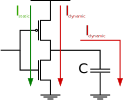
\includegraphics[width=0.5\textwidth]{figs/static-dynamic.pdf}
    \caption{Static and dynamic power through a PMOS and NMOS transistor}
    \label{fig:staticdynamic}
\end{figure}

\begin{figure}{tbh}
    \begin{subfigure}[b]{0.48\textwidth}
        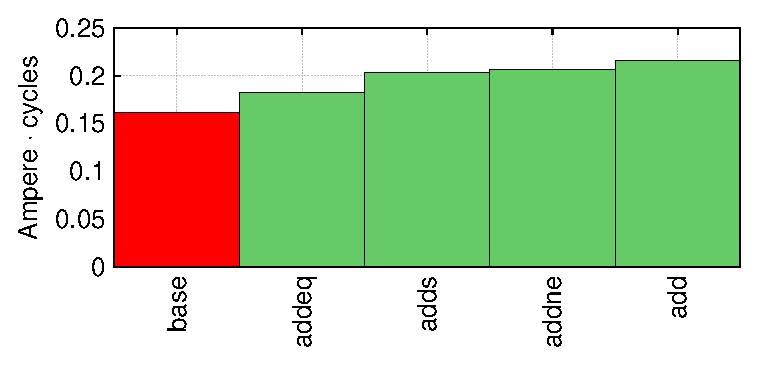
\includegraphics[width=\textwidth]{graph_01_base_cond-0c6.eps}
        \caption{Conditional execution (eq is false).}
        \label{fig:consumptioncond}
    \end{subfigure}
    \begin{subfigure}[b]{0.52\textwidth}
        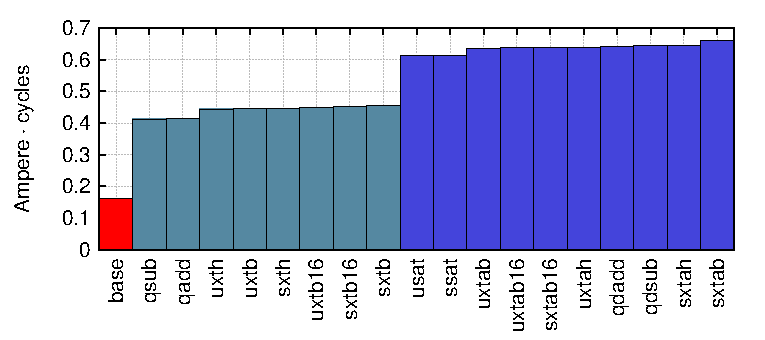
\includegraphics[width=\textwidth]{graph_023_base_quad_saturate_extend-0c6.eps}
        \caption{Non-multiply multi-cycle instructions.}
        \label{fig:consumptionmulti}
    \end{subfigure}
    \caption{Figures from \cite{rundehvatum2013exploring} showing the results of measuring the
    current drain through the CPU core while running isolated instructions in a loop.}
    \label{fig:consumption}
\end{figure}


